\section{Introduction}
\label{sec:introduction}

Currencies face both country-specific and global risks. This distinction is especially important for the carry trade. Diversification removes part of a currency's idiosyncratic risk, but it does not protect a portfolio that is long several high-interest-rate currencies when those currencies depreciate together. Because interest income accrues gradually, one shared exchange-rate movement can erase many months of carry. The empirical question is whether bond markets reveal such a state before the currency loss occurs.

An inversion of one country's yield curve is ambiguous. It may reflect domestic weakness, disinflation after a national tightening cycle, or a change in term premia. Synchronized inversions across several non-U.S. G10 economies are more likely to contain information about a global disturbance, although synchronization alone cannot distinguish global growth news from common policy or term-premium shocks. I combine fresh 10-year/2-year inversions across nine non-dollar G10 economies into a monthly state and ask whether that state predicts currency returns.

The construction is deliberately path dependent. A curve enters when it crosses into inversion and remains live until its slope has increased for two consecutive months. The synchronized-inversion state is active when at least two curves are live. Fresh entry separates new crossings from stale inversions; confirmed release keeps the state active when curves begin to re-steepen, including periods in which expected easing is being delivered. The state observed at the end of month $t$ predicts the return during month $t+1$.

The 1988--2026 sample contains 92 active months in fifteen episodes. Annualized carry-trade spot returns are 12.9 percentage points lower when the lagged state is active: 2.9 percent outside the state and $-10.0$ percent inside it. Total carry returns fall from 6.5 to $-4.9$ percent. The result is not only a label for the largest crashes. After removing each return series' full-sample bottom-decile months, the spot-return gap remains $-7.2$ percentage points per year. The center of the distribution also shifts: the monthly carry-spot median falls from 0.35 to $-0.76$ percent.

\begin{figure}[p]
    \centering
    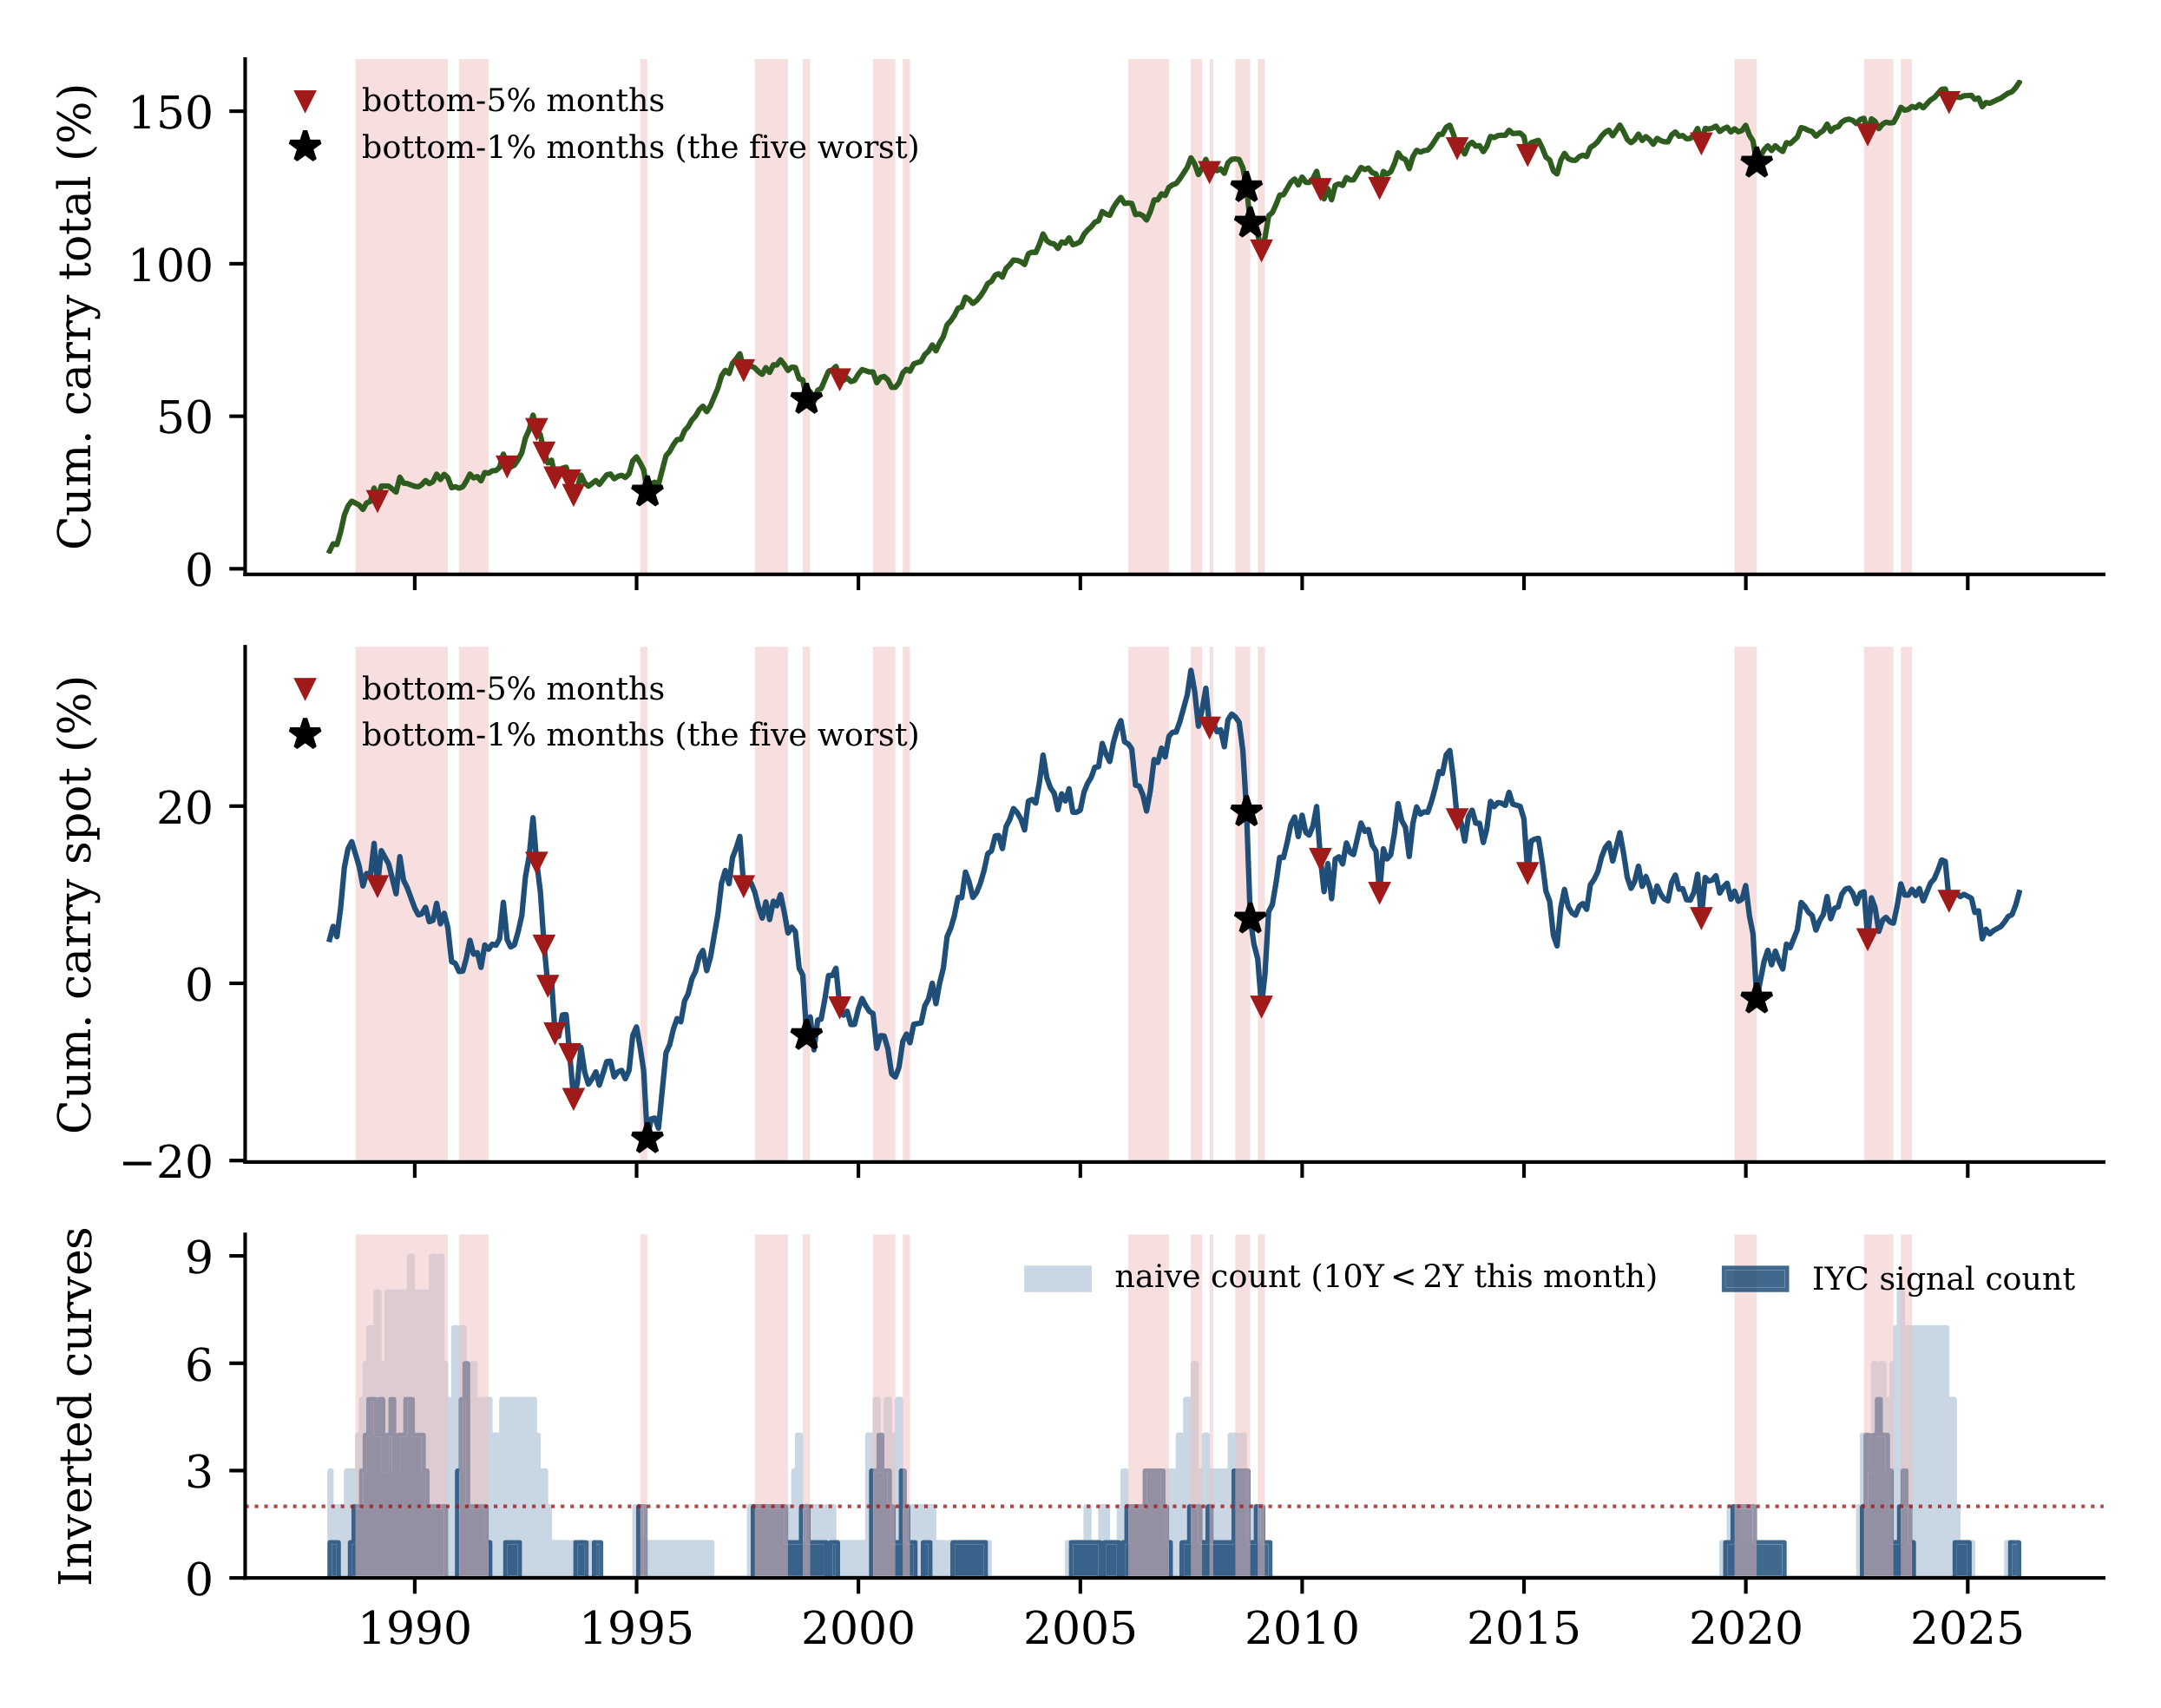
\includegraphics[width=\textwidth]{assets/original/figure_01_main.png}
    \caption{Carry returns and synchronized inversions. The light line counts curves currently inverted; the dark line counts fresh inversions that remain live under the release rule. The dotted line is the threshold of two. Shading denotes the end-of-month synchronized-inversion state, used with a one-month lag in every return regression. Tail markers show that the largest losses follow information already visible in the state, including episodes in which the current-inversion count has declined.}
    \label{fig:inherited_overview}
\end{figure}

The cross-section gives the result economic content. Carry buys high-interest-rate currencies and funds them with low-interest-rate currencies. Those rate rankings are correlated with exposure to global markets: the rank correlation between currencies' average interest differentials and their average predetermined equity betas is 0.72. In active-state months, high-rate currencies depreciate relative to low-rate currencies, and bilateral losses become larger as predetermined equity beta rises. Across nine currencies, the beta gradient explains 77 percent of the variation in estimated state coefficients; a portfolio formed directly on expanding-window equity betas loses 7.5 percentage points per year in spot returns in the state. The panel interaction has the expected negative sign but weak episode-level inference. Taken together, the estimates support an exposure ordering, not a precisely identified structural beta.

This ordering links two established literatures. National yield slopes forecast activity and reflect both expected short-rate paths and term premia \citep{harvey1988,estrellaHardouvelis1991,estrellaMishkin1998,campbellShiller1991,hamiltonKim2002}. International term structures also contain a shared component \citep{plosserRouwenhorst1994,bernardGerlach1998,diebold2008,chinnKucko2015}. The carry literature, meanwhile, shows that high-interest-rate currencies earn average premia but suffer negatively skewed losses in common stress states \citep{fama1984,brunnermeier2008,lustig2011,menkhoff2012,farhiGabaix2016}. The contribution here is to shift the unit of observation from one country's slope or a smooth global level factor to a cross-country configuration of fresh threshold crossings dated before the currency payoff.

The exposure ordering also clarifies why interest rates matter twice. The differential is the carry trade's known income, but it also ranks the currencies that bear the largest state-contingent spot losses. Commodity exposure, country size, trade-network position, and intermediary demand can all align high rates with sensitivity to global conditions \citep{hassan2013,ready2017,richmond2019,gabaixMaggiori2015}. The paper does not distinguish those channels. It shows that the loss is concentrated in currencies for which a predetermined market measure indicates greater exposure, rather than appearing as a uniform dollar movement.

Several results delimit this interpretation. One live inversion has the opposite return sign from two; the U.S. inversion alone has a small and imprecise coefficient; and the continuous average G10 slope, lagged financial conditions, and lagged VIX do not span the synchronized state. The five worst monthly carry returns occur under the lagged state, yet trimmed estimates and calendar splits show that 2008 and 2020 are not the entire result. These comparisons distinguish synchronization from nearby curve and risk measures. They do not identify the shock that synchronizes curves, and they do not remove the central design risk: the tenor, threshold, and release rule were assessed on the same historical sample.

Finally, a predictable negative conditional return is not an automatic implication of disaster exposure. In a frictionless benchmark, publicly known bad-state exposure should command compensation. The paper therefore treats slowly adjusting compensation as one candidate interpretation: fresh bond-market information can raise perceived loss risk before currency compensation fully adjusts. This mechanism explains why entry and timing may matter, but the return evidence does not identify the friction. The durable contribution is narrower and more testable: synchronized foreign yield-curve inversions predict where common currency losses subsequently occur.

Section~\ref{sec:setting} defines returns, the state, and timing. Sections~\ref{sec:design}--\ref{sec:main_evidence} present the design and evidence. Section~\ref{sec:mechanism} develops the exposure ordering and economic interpretation; Section~\ref{sec:robustness_limits} states the main limits. The online appendix gives the exact algorithm, derivations, supplementary estimates, and public-data checks.
